
%\section{Beyond Worst Case Analysis}

%In most cases, algorithms are characterized as ``good" or "bad" based on worst-case analysis, but there are examples that this characterization is not always accurate. Take the problem of Linear Programming, where the goal is to minimize (or maximize)  a linear objective function subject to linear constraints. Τwo algorithms solve this problem: the simplex method (exponential time in worst-case) and the ellipsoid method (polynomial in worst-case). Yet, empirically simplex performs way better than the ellipsoid method since worst-case instances are not ``real-world" instances. Another interesting example is the clustering problem, a well-known $NP$-hard problem. The goal is to partition a set of points into groups so that points in the same group are “similar” and those in different groups are “dissimilar”. The difficulty of the problem derives from the non-existent structure in the data in the worst-case instances, but these instances do not occur so often in the ”real world”.  In this section, we focus on the notion of stable instances in the sense that the optimal solution is ``well-defined" and small changes on the input will not affect the optimal solution.
%στο τέλος θέλει αλλαγή

%We have very negative results even in the line metrics, since there in no deterministic anonymous mechanism with bounded approximation for the $k$-Facility Location game with $k\ge3$.

%As we thoroughly discussed in the previous section, the Facility Location game is $NP$-Hard in the general setting.

Clustering and Facility Location games are two closely related problems. This is due to the fact that clustering, the primary optimization problem, and we know that is $NP$-Hard in general metric spaces. As we know very well, a problem is $NP$-Hard if no polynomial algorithm solves every input correctly. However, we are not interested in all instances but only those that appear in the real world. For clustering, it is cleverly stated in the paper by Bilu, Daniely, Linial, and Saks that  ``\emph{clustering is either easy or pointless}"\cite{bilu2012} and by Roughgarden,  ``\emph{clustering is hard when it doesn't matter}"\cite{Rough17_lect6}. But what does this actually mean? Clustering is the task of partitioning a set of points into groups so that points in the same group are ``similar" and those in different groups are ``dissimilar".  So in the ``real world", we expect that the clusters are well-defined, meaning that ``similar" points are relatively close to each other and far from any other point. This translates to communities or neighborhoods having ``clear borders" in the Facility Location game, making it easy to identify them and locate the facilities.  In the following section, we will refer to these instances as ``stable instances" and explore all the interesting properties of stability.

%We will also see how stability affects the design of algorithms and strategyproof mechanisms.


\section{Stable Clustering}


\begin{definition}[$k$-Clustering]
Given a set of points $X$ and a non-negative distance function $d: X\times X \rightarrow [ 0, \infty )$ a clustering $\vec{C} = (C_1,C_2,...,C_k)$ is the partitioning of the input points into k non-empty sets that minimizes an objective function:
\begin{enumerate}
    \item\textbf{The $k$-median objective}: minimize the sum of distances from points to their centers
    \[ \sum_{i=1}^{k} \left( \sum_{x\in C_i}  d(c_i,x)\right) \]
    \item\textbf{The $k$-center objective}: minimize the maximum distance of a point to its corresponding center
    \[ \max_{x_i \in C_i}  d(x_i,c_i)\]
\end{enumerate}
\end{definition}

%{??}
The $k$-median objective is equivalent to the social cost and the $k$-center to the maximum cost in the Facility Location game. 
\bigskip

We are moving to the formal definition of ``well-defined" or stable instances in clustering. Intuitively, stability means all points in the same cluster in the optimal solution are close together and that the clusters are well separated. It also means that the optimal solution is not affected by small changes in the input. We can perturb an instance to create nearby instances by scaling down the distance between any pair of points by a factor of at most $\g$, with $\g \ge 1$. 
\begin{definition}[$\g$-perturbation]
For $\g \ge$  1, a $\g$-perturbation of a metric space $(X, d)$ is
another space $(X, d')$ on the same point set such that:
\[ d'(x,y) \in \left[\frac{1}{\g}d(x,y),d(x,y)\right] \]
\end{definition}


\begin{definition}[$\g$-perturbation stability] \footnote{This definition does not state that the optimal cluster centers must remain the same.} 
A clustering instance $(X, d)$ is $\g$-perturbation stable to a given objective function $\Phi$ if there is a k-clustering $\vec{C}= C_1, . . . , C_k$ such that, for every $\g$-perturbation $(X, d')$, $\vec{C}$ remains the unique optimal k-clustering.
\end{definition}

There is also a weaker notion of stability called $\g$-\emph{metric perturbation stability}. In the definition of stability the perturbed space $d'$ does not need to be metric (i.e. $d'$ does not have to satisfy triangle inequality). In order for an instance to be $\g$-stable it needs to admit the same optimal solution in every $\g$-perturbation. For $\g$-metric stability we only require that the optimal solution remains the same for every $\g$-metric perturbation a subset of $\g$-perturbations. Thus, the class of $\g$-metric stable instances includes the class of $\g$-stable instances. The reason that we say $\g$-metric perturbation stability is a weaker notion of stability is because we relax the conditions for stability to more natural ones, therefore allowing more instances in that class.

\begin{definition}[$\g$-metric perturbation stability] \label{metricPer}
A clustering instance $(X, d)$ is $\g$-metric perturbation stable to a given objective function $\Phi$ if there is a k-clustering $\vec{C}= C_1, . . . , C_k$ such that, for every $\g$-metric perturbation $(X, d')$, $\vec{C}$ remains the unique optimal k-clustering.
\end{definition}


\section{Properties of Perturbation Stable Instances}


One of the most important properties for $\g$-stable instances is the \emph{center proximity} property which  implies that in the optimal solution every point is closer to its own center than to any other center.
\begin{definition}[$\g$-Center Proximity]\label{Cprox}
Let $\g \ge 1$, any $\g$-stable instance with unique optimal clustering $C_1, . . . , C_k$ and optimal centers $c_1, . . . , c_k$ satisfies $\g$-center proximity. For all distinct cluster pairs $C_i$ and $C_j$ and any point $x_i\in C_i$: 
\[d(x_i,c_j)>\g d(x_i,c_i) \]
\end{definition}
\begin{proof}
Let $C_i$ and $C_j$ be any two clusters in the optimal solution and $x_i \in C_i$. We consider a $\g$-perturbation of the original instance in which all distances among points in $C_i$ and points in $C_j$ are scaled down by a factor $\g$. Since this is a valid perturbation, the optimal clustering remains the same. Furthermore, since the distances within the clusters $C_i$ and $C_j$ are the same, $c_i$ remains the optimal cluster center for $C_i$ and $c_j$ for $C_j$. In the perturbed instance $x_i$ still belongs in $C_i$ so $d'(x_i,c_j) > d'(x_i,c_i)$. From the way the perturbed instance is created we have that $d'(x_i,c_j)=\frac{1}{\g} d(x_i,c_j)$ and that $d'(x_i,c_i) = d(x_i,c_i)$. Therefore,  $d(x_i,c_j) > \g d(x_i,c_i)$
\end{proof}

An immediate consequence of $\g$-center proximity  is that any point is $\g-1$ times closer to its own center than to any other point from a different cluster.

\begin{lemma}[$\g$-Weak Center Proximity]\label{WCprox}
Let $\g \ge 2$, any $\g$-stable instance with unique optimal clustering $C_1, . . . , C_k$ and optimal centers $c_1, . . . , c_k$ satisfies $\g-$weak center proximity. For any point $x\in C_i$ and $y \notin C_i$:
\[d(x,y)>(\g -1) d(x,c_i) \]
\end{lemma}

\begin{proof}
Let $x$ be any point in $C_i$ and $y$ any point in $C_j$. We need to distinguish two cases:
\begin{enumerate}[(i)]
    \item $d(y,c_j)\ge d(x,c_i)$: By triangle inequality we have that $d(y,c_i)\le d(y,x)+d(x,c_i)$. Since the instance is stable we have $d(y,c_i)>\g d(y,c_j)>\g d(x,c_i)$ from $\g$-center proximity property. Hence, we get that $d(x,y) \ge d(y,c_i) - d(x,c_i) > \g d(x,c_i) -d(x,c_i) = (\g-1) d(x,c_i)$
    \item $d(y,c_j) <  d(x,c_i)$: Again by triangle inequality we have that $d(x,c_j)\le d(x,y)+d(y,c_j)$. From $\g$-center proximity property we have $d(x,c_j)>\g d(x,c_i)$. Hence, we get that $d(x,y) \ge d(x,c_j) - d(y,c_j) > \g d(x,c_i) - d(x,c_i) = (\g-1) d(x,c_i)$
\end{enumerate}
\end{proof}

We can use the previous properties and show that the distance between any two points from a different cluster cannot be arbitrarily small.

\begin{lemma}[Cluster Separation Property]\label{CSprop}

Let $C_1, . . . , C_k$ be the optimal clustering of a $\g$-stable instance with $\g\ge2$. Let $x_i,x_i'\in C_i$ and $x_j \in C_j$ $(i\ne j)$ then:
\[ d(x_i,x_j) > \frac{(\g-1)^2}{2\g} d(x_i,x_i') \]
\end{lemma} 
\begin{proof}

Let $\CC$ be the optimal clustering of $\x$. Let $x_i,x_i'\in C_i$ have center $c_i$ and $x_j \in C_j$ $(i\ne j)$ have center $c_j$. We have that:
\begin{align}
\g d(x_i,c_i)&<d(x_i,c_j)<d(x_i,c_i) + d(c_i,c_j) \implies \nonumber \\
(\g-1)d(x_i,c_i)&<d(c_i,c_j) \label{dcenters}
\end{align}

Where the first inequality follows from the definition of the $\g$-center proximity and the second from the triangle inequality.
 We also have that:
 \begin{align}
     d(c_i,c_j)&<d(c_i,x_i)+d(x_i,x_j)+d(x_j,c_j)\nonumber \\
     &<\frac{2}{\g-1}d(x_i,x_j)+d(x_i,x_j)\nonumber \\
     &<\frac{\g+1}{\g-1}d(x_i,x_j)\label{dxi}
 \end{align}

Where the first inequality follows from the triangle inequality and the second from the definition of the $\g$-weak center proximity.
 
 \bigskip
 Finally we have that:

 \begin{align*}
    d(x_i,x_i') &\le d(x_i,c_i) + d(c_i,x_i')\\
    &\stackrel{(\ref{dcenters})}{<} \frac{1}{\g-1}d(x_i,x_j) + \frac{1}{\g-1}d(c_i,c_j)\\
    &\stackrel{(\ref{dxi})}{<} \frac{1}{\g-1}d(x_i,x_j) + \frac{\g+1}{(\g-1)^2}d(x_i,x_j) \\
    &= \frac{2\g}{(\g-1)^2}d(x_i,x_j)
 \end{align*}
 
\end{proof}



It is very important to note that the three properties presented above are necessary for stability but not sufficient. We can easily construct a non-stable instance in which all the properties hold. In the instance in figure \ref{fig:originalInstance} we can easily verify that all the inequalities are satisfied for $\g=3$ for any $\epsilon >0$. However, if we perturb the instance by scaling down the distances between agents $x_1-x_2$, $x_2-x_3$ and $x_3-x_4$ by a factor $\g$, the optimal clustering does not remain the same. On the left (figure \ref{fig:perOptCluster}) we have the same clustering as in the original instance. The cost of the left clustering is $\frac{2}{3}+4$. But if we place the centers as it is shown in the right (figure \ref{fig:diffCluster})  the cost is $4+\epsilon$. If the original instance was stable the optimal solution should have remained the same for all perturbations. Thus, the instance is not $3$-stable. 
%If we look closer we can see that this example  not a tight since the properties hold even if $d(x_3,x_4)=2+2\epsilon$.

\begin{figure}[ht]
     \centering
     \begin{subfigure}[b]{0.8\textwidth}
         \centering
         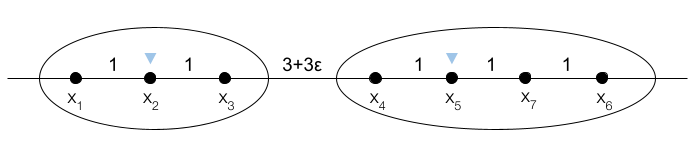
\includegraphics[width=\textwidth]{Images/nonStable1.png}
         \caption{Original instance.}
         \label{fig:originalInstance}
     \end{subfigure}
     \\
     \begin{subfigure}[b]{0.48\textwidth}
         \centering
         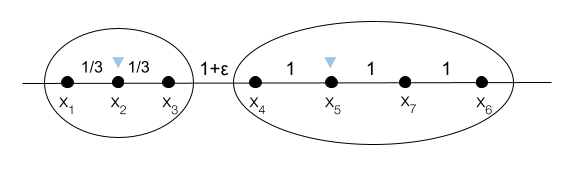
\includegraphics[width=\textwidth]{Images/nonStable2.png}
         \caption{Perturbed instance with the same clustering.}
         \label{fig:perOptCluster}
     \end{subfigure}
     \hfill
     \begin{subfigure}[b]{0.48\textwidth}
         \centering
         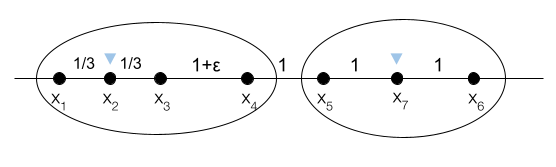
\includegraphics[width=\textwidth]{Images/nonStable3.png}
         \caption{Perturbed instance with an alternative clustering.}
         \label{fig:diffCluster}
     \end{subfigure}
      \caption{Example of non stable instance that satisfies all the properties.}
        \label{fig:NonStable}
\end{figure}



Never the less, the center-proximity is still a very important property. We can define the notion of $\g$-center stability. A instance is $\g$-center stable if in the optimal solution the center proximity holds for every point. This is a weak notion of stability since it allows more instances in the class. Figure \ref{fig:stability} illustrates all the different classes of stability.

\begin{definition}[$\g$-center stability]
A clustering instance $(X, d)$, with optimal solution $\CC= C_1, . . . , C_k$, is $\g$-center stable to a given objective function $\Phi$, if any $x_i\in C_i$ satisfies:
\[d(x_i,c_j) > \g d(x_i,c_i)\]
\end{definition}

\begin{figure}[ht]
    \centering
    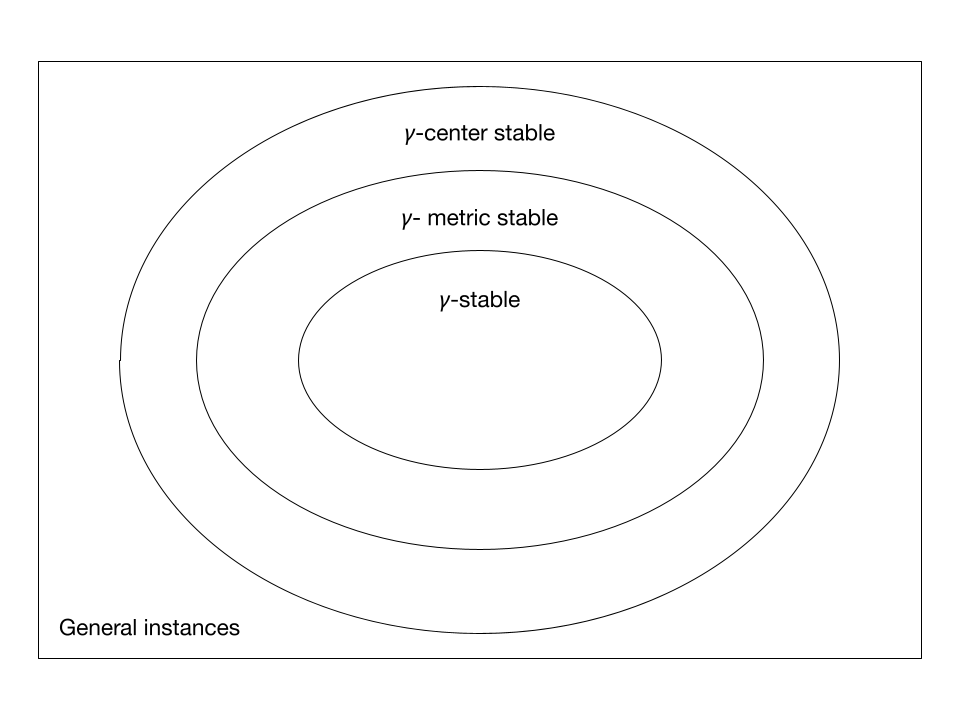
\includegraphics[width=11cm]{Images/stability.png}
    \caption{Classes of stable instances}
    \label{fig:stability}
\end{figure}




\section{Algorithms for Perturbation Stable Instances}

Τhe greater the factor of stability, the more structured the points are. For example, in every $2$-stable instance from weak center proximity, we get that every point is closer to its optimal center than any other point from  a different cluster. It is also very interesting that for a stability factor of $\g\ge2+\sqrt{3}\approx3.7$ we obtain from the separation property that all points are closer to all other points in their own cluster than to points in any other cluster. The next question is how we can use the properties derived from stability in order to achieve better results. The first idea is to see how existing algorithms perform on stable instances. \emph{Single-link} clustering is one of the most commonly used methods for clustering that uses the distances between the points. It starts with $n$ clusters of size $1$ (the data points), and at each step it merges the two clusters that have the minimum distance until there are $k$ clusters. One may think that if the instance is stable enough this algorithm could return the optimal solution, since at each step it connects the two ``closest" clusters. However, even in simple stable instances single linkage fails to find the optimal clustering. Consider an instance with 4 distinct locations $\x=(x_1,x_2,x_3,x_4)$. Our goal is to place $3$ facilities. There is one agent located at $x_1$ and $M>>1$ agents located at every other location. 

\begin{figure}[ht]
    \centering
    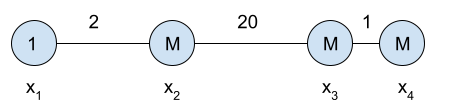
\includegraphics[width=13cm]{Images/SingleLinkageC.png}
    \caption{An example that single linkage fails to find the optimal solution}
    \label{fig:signleLinkage}
\end{figure}

The optimal solution is to place the centers at $x_2,x_3$ and $x_4$ and connect $x_1$ to the center at $x_2$. The total cost of the optimal solution is $2$. But the single-linkage clustering will merge the the clusters at $x_3$ and $x_4$ and places one center between them making total cost of the solution equal to $M$, which is arbitrarily larger than the optimal cost. Note that by construction the instance is $\g$-stable for arbitrarily large $\g$, for a properly selected value of $M$.  

But a variation of the previous algorithm can find the optimal solution for a sufficient $\g$ stability. It starts with $n$ clusters of size $1$. Instead of stopping at $k$ clusters it continues until one cluster remains. Then it finds the best $k$ clusters of the resulting tree $T$ using dynamic programming. 
%{?Write the dp?}

\begin{lemma}\label{sl}
Single linkage can find the optimal solution if and only if each cluster forms a subtree of the spanning tree. 
\end{lemma}

\begin{proof}
The single linkage algorithm outputs the best $k$-clustering among all the $\binom{n-1}{k-1}$ different choices. Every different clustering can be obtained by removing $k-1$ edges from the spanning tree. This way all the $k$ clusters are different connected components of  $T$, If some optimal cluster is not a connected subgraph of T the algorithm cannot find it.
\end{proof}
This can be illustrated with a simple example. 

\begin{figure}[ht]
    \centering
    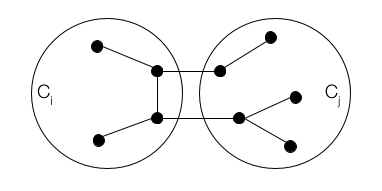
\includegraphics[width=9cm]{Images/MST.png}
    \caption{The optimal cluster $C_j$ do not form a subtree of $T$}
    \label{fig:my_label}
\end{figure}


The function used to determine the distance between two clusters, is known as the linkage function. For different functions we get different stability factors for which we can find the optimal solution. 

%--------------------------------------------------
% 3 & 2+sqrt(3)
The first linkage function was proposed by Awasthi \cite{Awasthi2012}. At each step it merges the two cluster $C,C'$ minimizing $d_{min}(C,C')$. The minimum distance between any two subsets $A,B \subset X$ is defined as:
\[ d_{min}(A,B) = min \{ d(a,b) | a\in A, b\in B\} \]

They prove that the single-linkage algorithm can return the optimal solution for a stability factor $3$ when centers must be data points and for stability factor $2+\sqrt{3}$ for general metrics. With tighter analysis Angelidakis showed \cite{Angelidakis2017} that the instance only needs to be $2$-metric stable, when the centers must be data points.

%From the Lemma \ref{sl}
\begin{lemma}
Single-linkage with $d_{min}$ as the linkage function finds the optimal solution in every $2$-metric stable instance. 
\end{lemma}

\begin{proof}
By Lemma \ref{sl} if every optimal cluster $C_i$ is a connected subgraph on the spanning tree $T$ then single-linkage returns the optimal solution. It is enough to show that the unique path that connects any point $a \in C_i$ to its optimal center $c_i$ on $T$ does not leave the cluster $C_i$. Suppose that $b$ is the next point on the path. Consider the step at which the single-linkage adds the edge $(a,b)$ to the spanning tree. At that step, $a$ and $c_i$ belonged in different clusters, otherwise the edge $(a,b)$ would form a cycle. We have that $d(a,b)<d(a,c_i)$ or else the edge $(a,c_i)$ would have been added instead of $(a,b)$. By Lemma \ref{WCprox} the previous inequality implies that $b$ belongs to $C_i$.  By induction all the points on the path between $a$ and $c_i$ belong to $C_i$.  
\end{proof}





%--------------------------------------------------
% 1+sqrt(2) center

The second linkage function was proposed by Balcan and Linang \cite{Balcan2011}. The single linkage algorithm merges the clusters with the minimum closure distance. The closure distance between two clusters $C,C'$ is the radius of the minimum ball that covers all the points in $C \cup C'$ and has some margin from points outside of the ball. A ball around $p$ with radius $r$ is set of all points that have distance from $p$ smaller than $r$: $\mathbb{B}(p,r) \coloneqq \{ q : d(p,q) <r \}$ 


\begin{definition}[Closure Distance]
The closure distance $d_S(C,C')$ between two disjoint nonempty subsets $C,C' \subset X$ is the minimum $d>0$ such that there is a point $c\in C\cup C'$ satisfying the following requirements:
\begin{enumerate}[(i)]
    \item Coverage: the ball $\mathbb{B}(c,d)$ covers $C$ and $C'$, that is, $C\cup C' \subseteq \mathbb{B}(c,d)$ 
    \item margin: points inside $\mathbb{B}(c,d)$ are closer to the center c than to points outside, that is, $\forall p \in \mathbb{B}(c,d), q\notin \mathbb{B}(c,d)$, we have $d(c,p)<d(c,q)$
\end{enumerate}

\end{definition}
\begin{lemma}
Single-linkage with $d_S$ as the linkage function finds the optimal solution in every $1+\sqrt{2}$-center stable instance. 
\end{lemma}

%\begin{proof}
%??????????
%\end{proof}

%This technique works because at each step every connected component is either a subset of a cluster in C, equal to C or a union of clusters in C. This is because the instance is stable and the algorithm always prefers to connect points that belong in the same cluster before connecting points from different clusters.




\section{Conclusion}

%Lower bounds
%approx stability 
%neg cant find how stable an instance is


Using the techniques from \emph{Beyond Worst Case Analysis} helps us avoid the hardness results in the general case. For clustering, we are able to design exact algorithms for a problem that is NP-hard to even approximate. However, the notion of perturbation stability does not completely solves our problem. There is an NP-hardness lower bound for the stability factor. For any $\epsilon>0$, finding the optimal $k$-center clustering for $(2-\epsilon)$-perturbation stable instances is $NP$-hard, unless $NP=PR$\cite{Balcan2015}. We also have that is $NP$-hard to find the optimal $k$-median clustering for $(2-\epsilon)$-center stable instances \cite{Ben-David2014}. Since the single-linkage algorithm only relies on the center proximity, which means the previous algorithm is tight. However, the class of $\g$-stable instances is a subclass of $\g$-center stable instances, which means that the lower bound does not transfer immediately. To show a lower bound for the class of $\g$-stable instances or to find a better algorithm, we need a different approach, specifically to include valid perturbations.

One downside of this approach is that there is no algorithm that can find or even estimate the  $\g$ for which an instance is $\g$-stable. However, the notion of $\g$-perturbation stability is still very important because it captures all the instances that have a ``clearly optimal" solution. That means we are clustering with the correct objective, which is not susceptible to minor perturbations.

%The class of $\g$-center stable instances includes all the instances for which in the optimal solution the $\g$-center proximity property holds. The class of $\g$-center stable instances includes the class of $\g$-perturbation stable instances since $\g$-center proximity is a necessary property for stability but not sufficient. ++++

%$(\g,\epsilon)$-perturbation stability, which states that at most a fraction $\epsilon$ of the total points can change cluster under any $\g$-perturbation.




